\documentclass[letterpaper, 12pt, conference]{ieeeconf}
\IEEEoverridecommandlockouts
\overrideIEEEmargins

\usepackage{tikz, circuitikz}
\usetikzlibrary{positioning}

%In case you encounter the following error:
%Error 1010 The PDF file may be corrupt (unable to open PDF file) OR
%Error 1000 An error occurred while parsing a contents stream. Unable to analyze the PDF file.
%This is a known problem with pdfLaTeX conversion filter. The file cannot be opened with acrobat reader
%Please use one of the alternatives below to circumvent this error by uncommenting one or the other
%\pdfobjcompresslevel=0
%\pdfminorversion=4

% See the \addtolength command later in the file to balance the column lengths
% on the last page of the document

% The following packages can be found on http:\\www.ctan.org
%\usepackage{graphics} % for pdf, bitmapped graphics files
%\usepackage{epsfig} % for postscript graphics files
%\usepackage{mathptmx} % assumes new font selection scheme installed
%\usepackage{times} % assumes new font selection scheme installed
%\usepackage{amsmath} % assumes amsmath package installed
%\usepackage{amssymb}  % assumes amsmath package installed

\title{\LARGE \bf
COM S 336 Ray Tracer Final Report
}

\author{Michael Drobot}

\begin{document}

\maketitle
\thispagestyle{empty}
\pagestyle{empty}

\begin{abstract}
The COM S 336 course project is a software ray traced graphics engine that supports a variety of features. This implementation is written in C++. It supports quads, quadrics, depth of field, instancing, Perlin noise, and parallelization on top of the required feature set.
\end{abstract}

\section{INTRODUCTION}

The COM S 336 final project is a software-implemented ray trace engine. This implementation supports a variety of features (listed below). It is written in C++ with object-oriented styling. The ray tracer can be configured through command-line options and through a scene file, written in JSON \cite{nlohmannjson}. The command-line options configure the environment and render engine while the scene file configures the camera and the objects in the scene.

This project relied heavily on the math and information provided in Shirley, Black, and Hollasch's Ray Tracing in One Weekend series \cite{Shirley2025RTW1} \cite{Shirley2025RTW2}.

\begin{itemize}
    \item Required features
    \begin{itemize}
        \item Camera positionable in all 6 degrees of freedom with variable field of view
        \item Anti-aliasing
        \item Spheres, with or without textures
        \item Triangles, with or without textures
        \item Texture loading from files
        \item Triangle mesh (model) loading from files
        \item A spacial subdivision acceleration structure
        \item Specular, diffuse, dielectric, and emissive materials
    \end{itemize}
    \item Additional required features chosen by me
    \begin{itemize}
        \item Quads
        \item Parallelization
        \item Object instancing
    \end{itemize}
    \item Additional non-required features
    \begin{itemize}
        \item Quadrics
        \item Perlin noise
        \item Depth of field (defocus blur)
    \end{itemize}
\end{itemize}

\section{INTERFACE}
The ray tracer provides two interfaces to the user: command-line configurations and the scene JSON file. Command-line flags are used to configure the rasterizer, runtime environment, and provide a scene file. The helptext can be viewed by running \verb|render.exe -h|.

The scene JSON file contains configurations for the camera and for each object in the scene. Certain values take paths, paths should be relative to the working directory where the renderer was run. The sample files provided contain the exact JSON tags to use when configuring an object, but a summary is shown below. Comments aren't allowed in JSON files, so "comments" should be added in a tag called \verb|"_comment"|.

\begin{verbatim}
{
    "_comment": "A comment",
    "type": "triangle", "sphere",
            "quad", "quadric",
            or "obj",
    "surface": "specular", "diffuse",
               "dielectric",
               or "emissive",
    "texture": "hexColorCode" or
               "pathToTextureFile",
    "perlin": true or false,
    "someObjectSpecificConfig": 1234
}
\end{verbatim}

\section{CONVENTIONS AND MATH}
Rays are expressed in terms of an origin point, a normalized direction vector, and a time parameter. All direction and normal vectors will be normalized, both in the source code and in this document.

\begin{center}
    \[
        P(t) = O + tD
    \]
\end{center}

\section{CAMERA}
The camera is the starting point for all rays in the scene. It is fully configurable and posable through the scene JSON file. All degrees of freedom can be determined with an origin point (corresponding to the middle of the image plane), a top vector, and a front vector. It should be noted that there is a difference between the image plane, the pinhole, and the lens: the image plane is where image samples are captured, the lens and the pinhole are where rays originate from. This is shown in Figure \ref{fig:camera}.

\begin{figure}
    \centering
    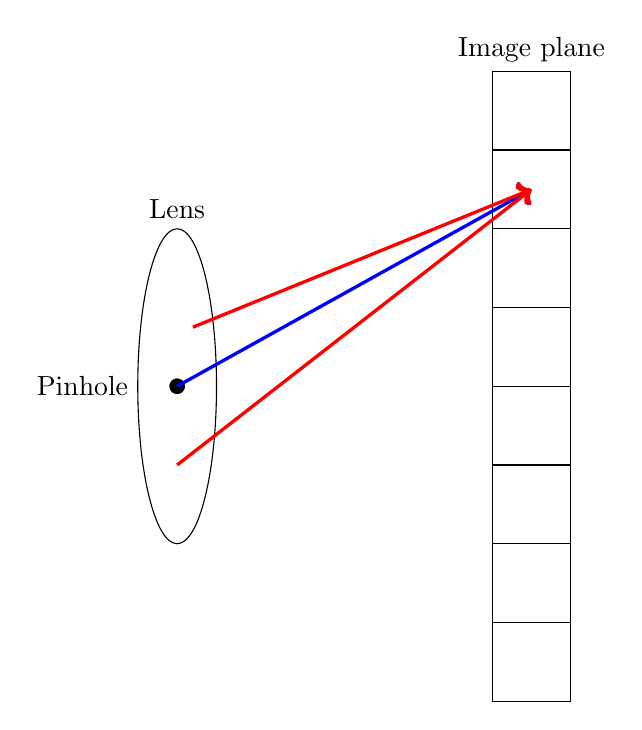
\begin{tikzpicture}
        % Blocks
        \draw (0, 2) ellipse (0.5cm and 2cm) node[anchor=south, yshift=2cm]{Lens};
        \fill[black] (0, 2) circle (0.1cm) node[anchor=east, xshift=-0.5cm]{Pinhole};
        \draw[step=1cm,black] (4, -2) grid (5,6) node[anchor=south, xshift=-0.5cm]{Image plane};

        % Arrows
        \draw[very thick,->, blue] (0, 2) -- (4.5, 4.5);
        \draw[very thick,->, red] (0.2, 2.75) -- (4.5, 4.5);
        \draw[very thick,->, red] (0, 1) -- (4.5, 4.5);
    \end{tikzpicture}
    \caption{The camera model}
    \label{fig:camera}
\end{figure}

The scene file specifies the location of the image plane because it's the most relevant part of the camera: it's where the colors are captured. Specifying the location of the lens or pinhole location is also valid, but that introduces some confusion when precisely positioning the camera. The camera can be positioned to "take a picure" outside of a room, but after accounting for the focal distance it ends up recording the inside of the room. It's more useful to specify exactly where the picture will be taken.

The image plane is a \verb|aspect_ratio x 1| rectangle centered on the specified origin point. This rectangle is subdivided into the pixels that make up the finished image. When rays are initialized the renderer picks a random location inside the pixel and calculates the vector from the pinhole to it (call that vector $V$, shown in blue in Figure \ref{fig:camera}). The resulting ray's origin is set to the intersection point between $V$ and the image plane, and the resulting direction is $norm(V)$.

Anti-aliasing (reducing the "blockiness" in a final render) is achieved by running this procedure hundreds or thousands of times. The randomness in the ray entering the scene helps blur edges and remove aliasing.

Depth of field, or defocus blur, is done by expanding the pinhole to a disk-shaped lens. Instead of choosing a random point in a pixel on the image plane we choose a random point on the lens and shoot the ray through the center of the pixel on the image plane (shown in red in Figure \ref{fig:camera}). This is the thin lens approximation technique, and can be used to add bokeh around objects in front or behind of the focus plane.

\section{LOADING AND INSTANCING}
Simple objects (triangles, spheres, quads, quadrics) are specified entirely through the scene file. However, complex triangle meshes are better loaded from standard file formats like Wavefront OBJ. This ray tracer uses the tinyobjloader library to parse OBJ files into C++ objects \cite{tinyobjloader}. Each model is rotatable and scalable using parameters in the scene file. Instancing is handled by only loading each OBJ model file once and applying the transformations specified in the scene file.

\section{INTERSECTIONS}
At this moment the scene has rays and geometry. Now the rays need to interact with the geometry.

The core principle of a ray tracer is to \textbf{find the closest point the ray hits for any given ray}. This means intersection tests need to be computed for every object for every bounce of every ray in the scene. While the intersection tests are simple the sheer number of tests means it's very computationally intensive. Significant time was spent ensuring that intersection tests performed well. A much more significant performance increase can be had with a spacial acceleration structure, discussed later on.

Triangles are represented by their vertex locations and the winding order (determines which side is "up" by right-hand rule). Intersections were computed in two steps. First, a plane intersection test checks if the incoming ray hits the plane containing the triangle. A miss could mean a ray going in the opposite direction or parallel to the plane. If the first test passes, an "outside-inside" test is run using barycentric coordinates. If all barycentric coordinates are positive then the ray intersects the inside of the triangle. The normal vector is computed using the winding order.

Triangle meshes are simply a set of triangles. They're represented as vertex and index buffers, where each element in the index buffer is a triangle (represented as a set of 3 vertex buffer indices). After looking up the triangle's vertices in the vertex buffer the ray tracer constructs a triangle and runs an intersection test as normal.

Quadrics and spheres (a subset of quadrics) can be defined with the equation shown below. After substituting the parameterized equation for each vector and reorganizing into standard quadratic equation form with respect to $t$ it can be plugged into the quadratic formula and solved. No real solutions (negative discriminant) indicate a miss, one real solution (discriminant = 0) indicate a grazed hit, and two real solutions (positive discriminant) indicate a pass through. Note that we only care about the \textbf{closest} hit, so pick the negative side of the $\pm$.

In reality, sphere intersections are slightly more optimized than the equations shown below. They are used often enough to justify a more optimized implementation. This is discussed in more detail in Ray Tracing in One Weekend \cite{Shirley2025RTW1}. The normal vector is computed using the radius of the sphere.

Quadrics can be used to make any derivative of a hyperboloid function (primarily cones and cylinders). They are fully parameterized and take in $a^2, b^2, c^2, d^2$. Quadrics are reflected across a particular axis and we only want one side of the reflection. The intersection test is very similar but there is an additional bounding box check. The normal vector is computed using the gradient of the surface at the intersection point.

\begin{center}
    \[
    \frac{(C_x - X)^2}{a^2} + \frac{(C_y - Y)^2}{b^2} + \frac{(C_z - Z)^2}{c^2} = d^2
    \]
    where
    \[
    X = O_x + t D_x
    \]
    \[
    Y = O_y + t D_y
    \]
    \[
    Z = O_z + t D_z
    \]
\end{center}

Quads consist of an origin point, a width vector, and a height vector. Intersection tests are completed in two steps, similar to triangles. First, the same plane intersection test checks if the ray hits the plane containing the quad. Second, an "outside-inside" test checks if the ray hit inside the quad. The inside-outside test is done with a change of basis, explained in more detail in Ray Tracing in One Weekend \cite{Shirley2025RTW2}. The normal vector is computed using the cross product of the width and height.

\section{MATERIALS}
There are four materials supported by this ray tracer: diffuse (dull, matte), specular (mirrored, reflective, metallic), dielectric (water, gemstones), and emissive (light sources). After performing an intersection test and confirming a hit the ray tracer will calculate the color and direction of the ray that bounces off of the surface.

Diffuse surfaces attenuate and scatter light. Attenuation happens because, for example, a red surface only reflects red light. All other wavelengths are absorbed. The attenuation is calculated by multiplying the surface's color by the incoming ray's color. Scattering is simulated by randomizing the the reflected ray's direction.

Specular surfaces are perfectly reflective. They don't attenuate light and they have perfect reflection directions. The reflected ray's color is equal to the incoming ray. The reflected ray's angle relative to the normal vector is equal to the incoming ray.

Dielectric surfaces have a probability of reflecting or refracting (bending) light. This follows the index of refraction of the object hit and which side the object is hit from (inside or outside).

\section{TEXTURES}
Textures are solid colors read from the scene file, images loaded from the filesystem, or one of the above with Perlin noise applied. Textures are only applied to diffuse surfaces. Solid colors are trivial, so we will focus on image loading and Perlin noise.

Images are loaded from disk and each axis is mapped to the range $[0, 1]$ \cite{stb}. In graphics these are referred to as texture coordinates, texcoords, or $u, v$ coordinates.

Triangle barycentric coordinates map easily: take a weighted average of each vertex's texture coordinate and its barycentric coordinate.

Spheres also map easily: convert the intersection point on the sphere's surface to spherical coordinates and rescale $\phi$ and $\theta$ to match the range of $u, v$.

Quads are even easier: the inside-outside test gives the intersection point in terms of the width and height vectors, these are equivalent to the $u, v$ coordinates.

Perlin noise generates a random map of floating point values corresponding to each point in 3D space. This is useful for terrain generation, natural-looking patterns, fire, and fog. In this ray tracer it was only used for texture generation. The Perlin noise generation returns a value in the range $[0, 1]$. Multiply the noise value by the color of any intersection on any diffuse object to apply the noise.

\section{BOUNDING VOLUME HIERARCHIES}
Spatial acceleration structures greatly improve performance of ray tracers by reducing the number of complex object intersection tests that need to be performed. The bounding volume hierarchy structure places each primitive object into a axis-aligned bounding box and orders the bounding boxes into a binary tree. The tree construction requires that each bounding box must be entirely contained in its parent bounding box and each leaf node must contain only one primitive.

Each ray will traverse the tree, testing for intersection with each bounding box it reaches. Eventually it will reach a leaf node, containing a primitive to run an intersection test against. Bounding box intersection tests are much cheaper than object intersection tests, so even though the total intersection test count has increased the overall computation time has decreased.

A ray may hit multiple bounding boxes. Therefore, while traversing the BVH the execution must keep track of the closest primitive hit. The traversal only returns the closest primitive hit.

\section{PERFORMANCE}
Performance is hard to quantify. There are too many variables in the machine used to run the program, the underlying OS, and the compiler and compiler settings. This ray tracer completes the Cornell box sample scene provided with the source code using the specs below in 3 hours and 45 minutes. The program can definitely be optimized further, but that is beyond the time I have for this project.

\begin{itemize}
    \item Resolution: 1920 x 1080
    \item Rays/pixel: 1000
    \item Ray bounce depth: 50
    \item Job count: 18
    \item CPU: AMD Ryzen 7 5825U 8c16t, 15W TDP
    \item RAM: 16GB
\end{itemize}

\section{CONCLUSIONS}
\begin{figure}[h!]
    \centering
    \includegraphics[width=0.9\linewidth]{final_render.png}
    \caption{Final render (cornell\_box.json)}
    \label{fig:final_render}
\end{figure}

This implementation of the COM S 336 ray tracer project has additional functionality and quality of life features above the base required elements. It supports a variety of geometry, surface textures, materials, and performance improvements. This project has been one of the most interesting programming adventures I've had in my career at Iowa State. It fits well with my passion for graphics and practical implementation. The final product performs well and I hope to improve it further in the future.

\addtolength{\textheight}{-12cm}

\bibliographystyle{IEEEtran}
\bibliography{bib}

\end{document}
